\chapter{Your Central Work}

Always put text between section titles.

\section{Section}

\begin{lstlisting}[mathescape]
$i$ := $0$;
$j$ := $\frac{n}{2}$;
while $i$ $\leq$ $\frac{n}{2}$ and $j$ $\geq$ $0$ do
	if $l_x$[$i$] = b or $l_y$[$j$] = b then
		return true;
	end
	if $l_x$[$i$] + $l_y$[$j$] < b then
		$i$ := $i$ + $1$;
	else if $l_x$[$i$] + $l_y$[$j$] > b then
		$j$ := $j$ - $1$;
	else
		return true;
	end
end
return false;
\end{lstlisting}


\subsection{Another Subsection}

\begin{table}
    \centering
		\caption[Flammkuchenteig]{Flammkuchenteig. The ingredients have to be carefully chosen.\label{tab:mytable}}
    \begin{tabular}{|l|p{0.4\linewidth}|}
    \hline
    \emph{Quant.} & \emph{Ingredient}\\
    \hline
		200g &Wei{\ss}mehl\\
		1/4  &Packung Frischhefe\\
		4EL  &lauwarme Milch\\
		4EL  &Öl\\
		1TL  &Zucker\\
		1TL  &Salz\\
		&lauwarmes Wasser\\
    \hline
    \end{tabular}    
\end{table}

\subsection{More Subsections}


\begin{figure}[htb]
     \centering
     \subfloat[][Caption first]{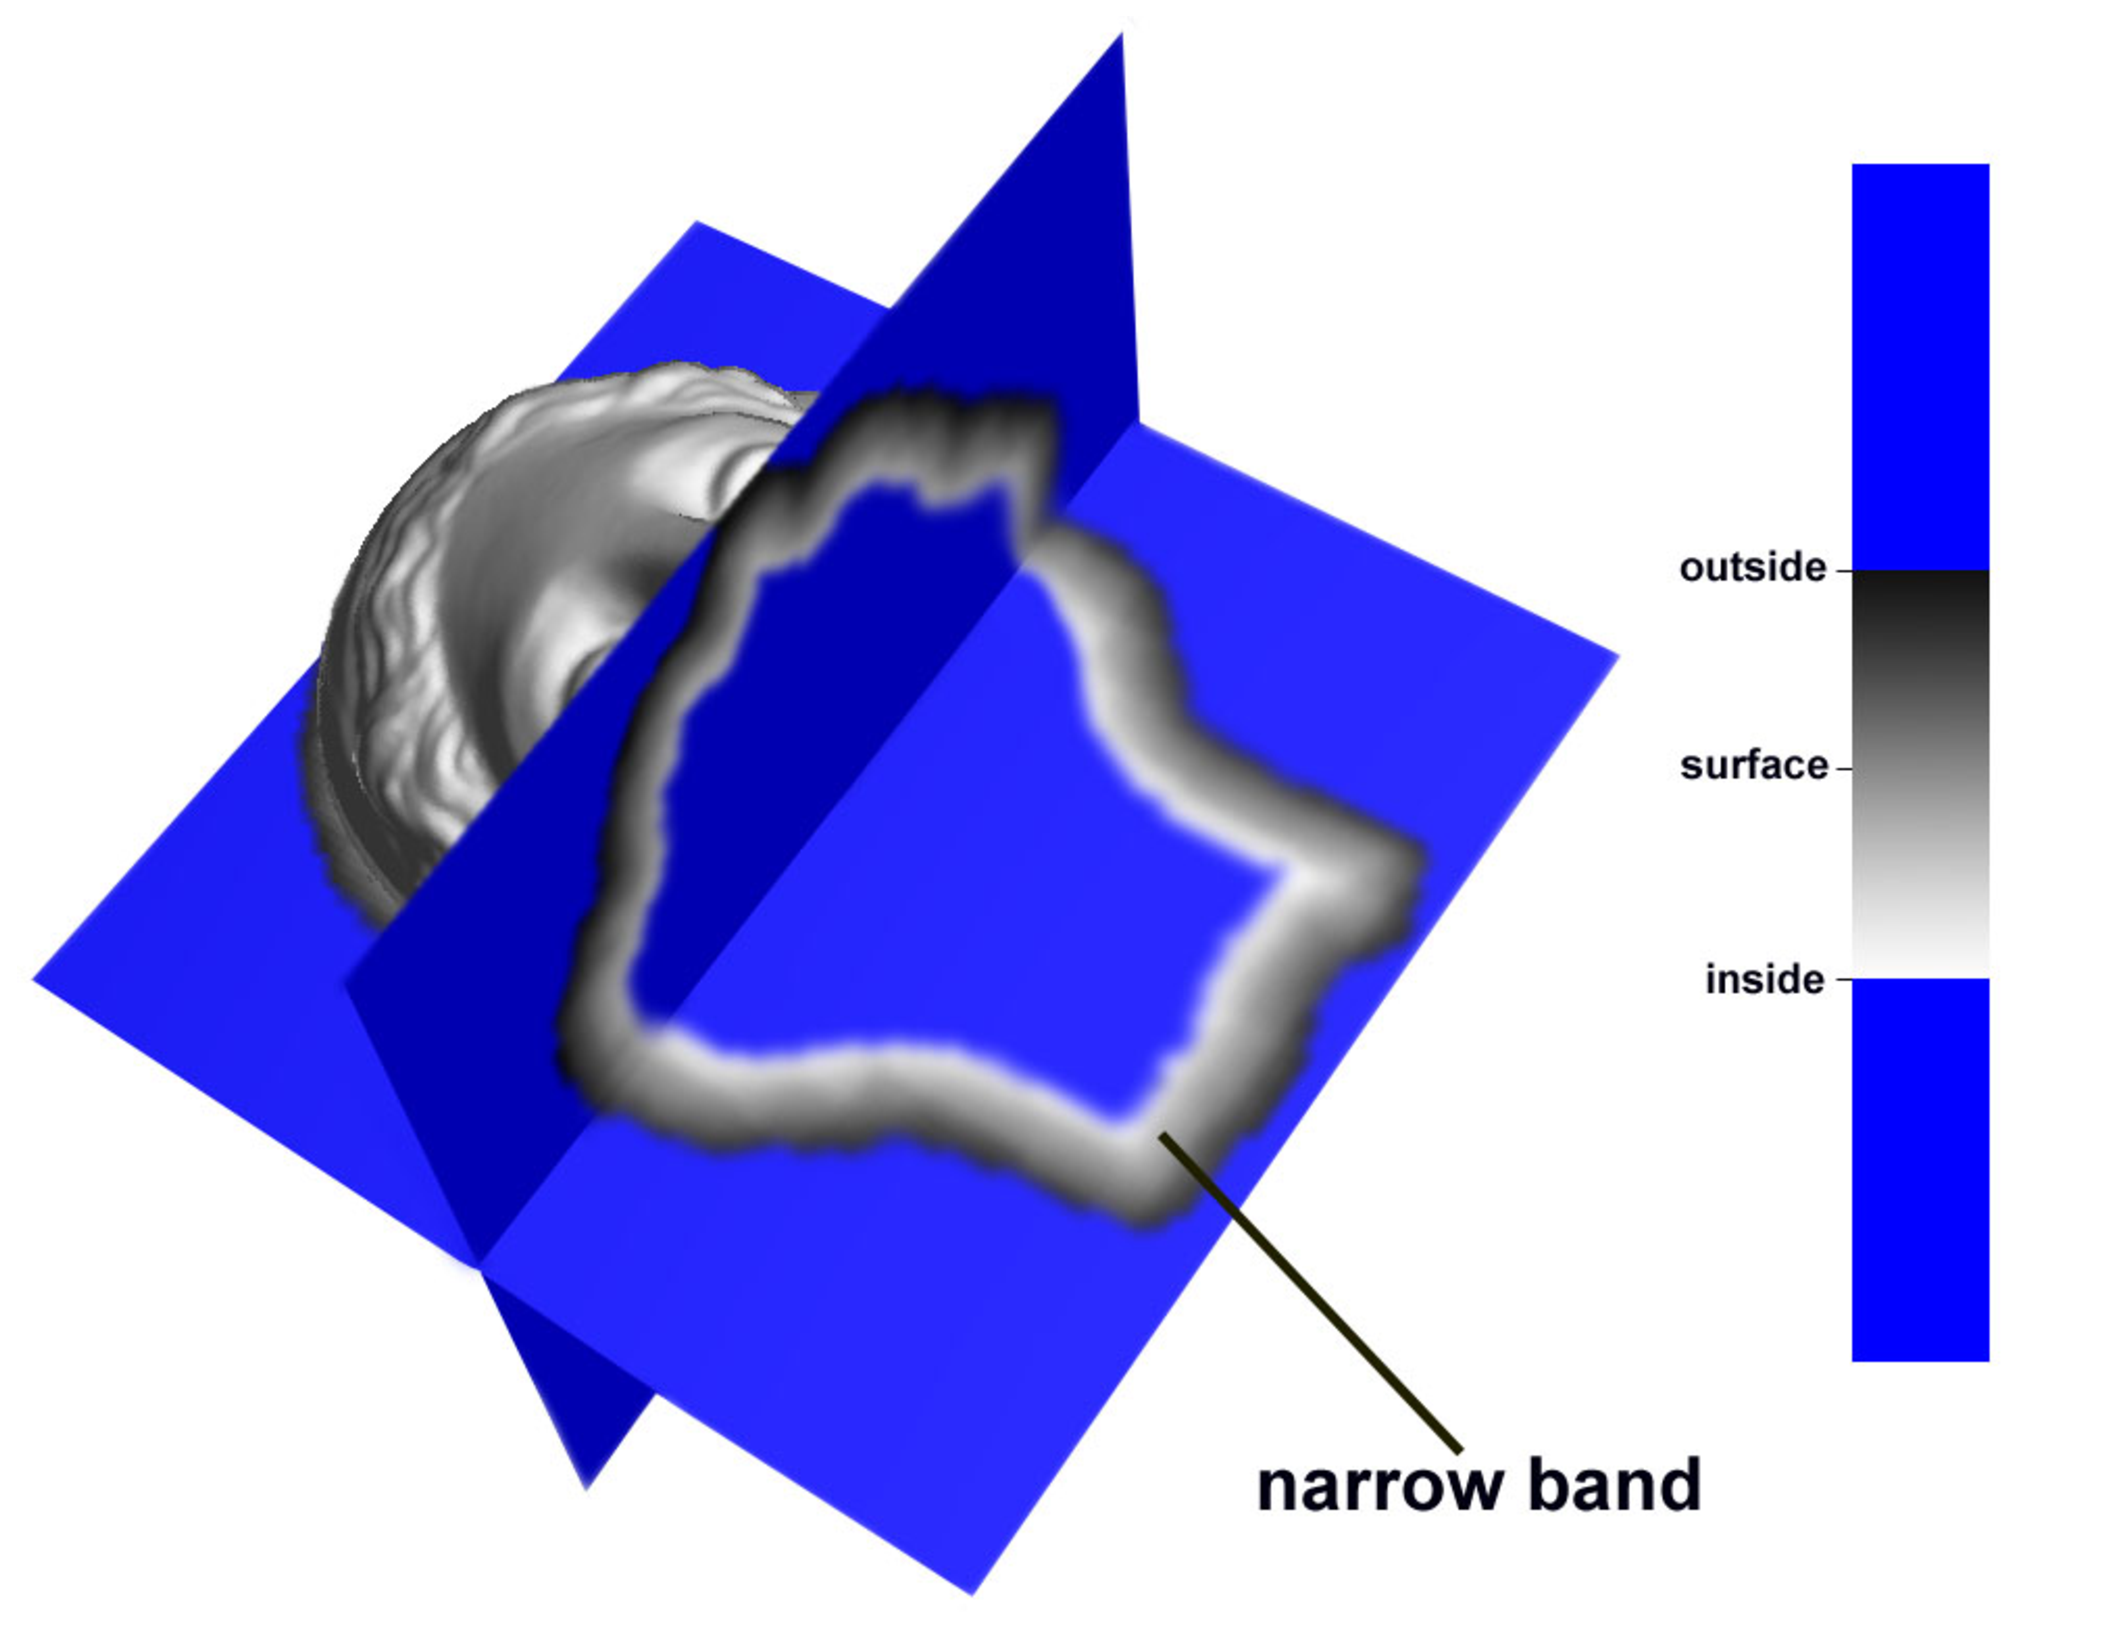
\includegraphics[width=0.45\textwidth]{figures/IgeaNarrowBand}\label{fig:twofigures:IgeaNarrowBand}}
     \subfloat[][Caption first]{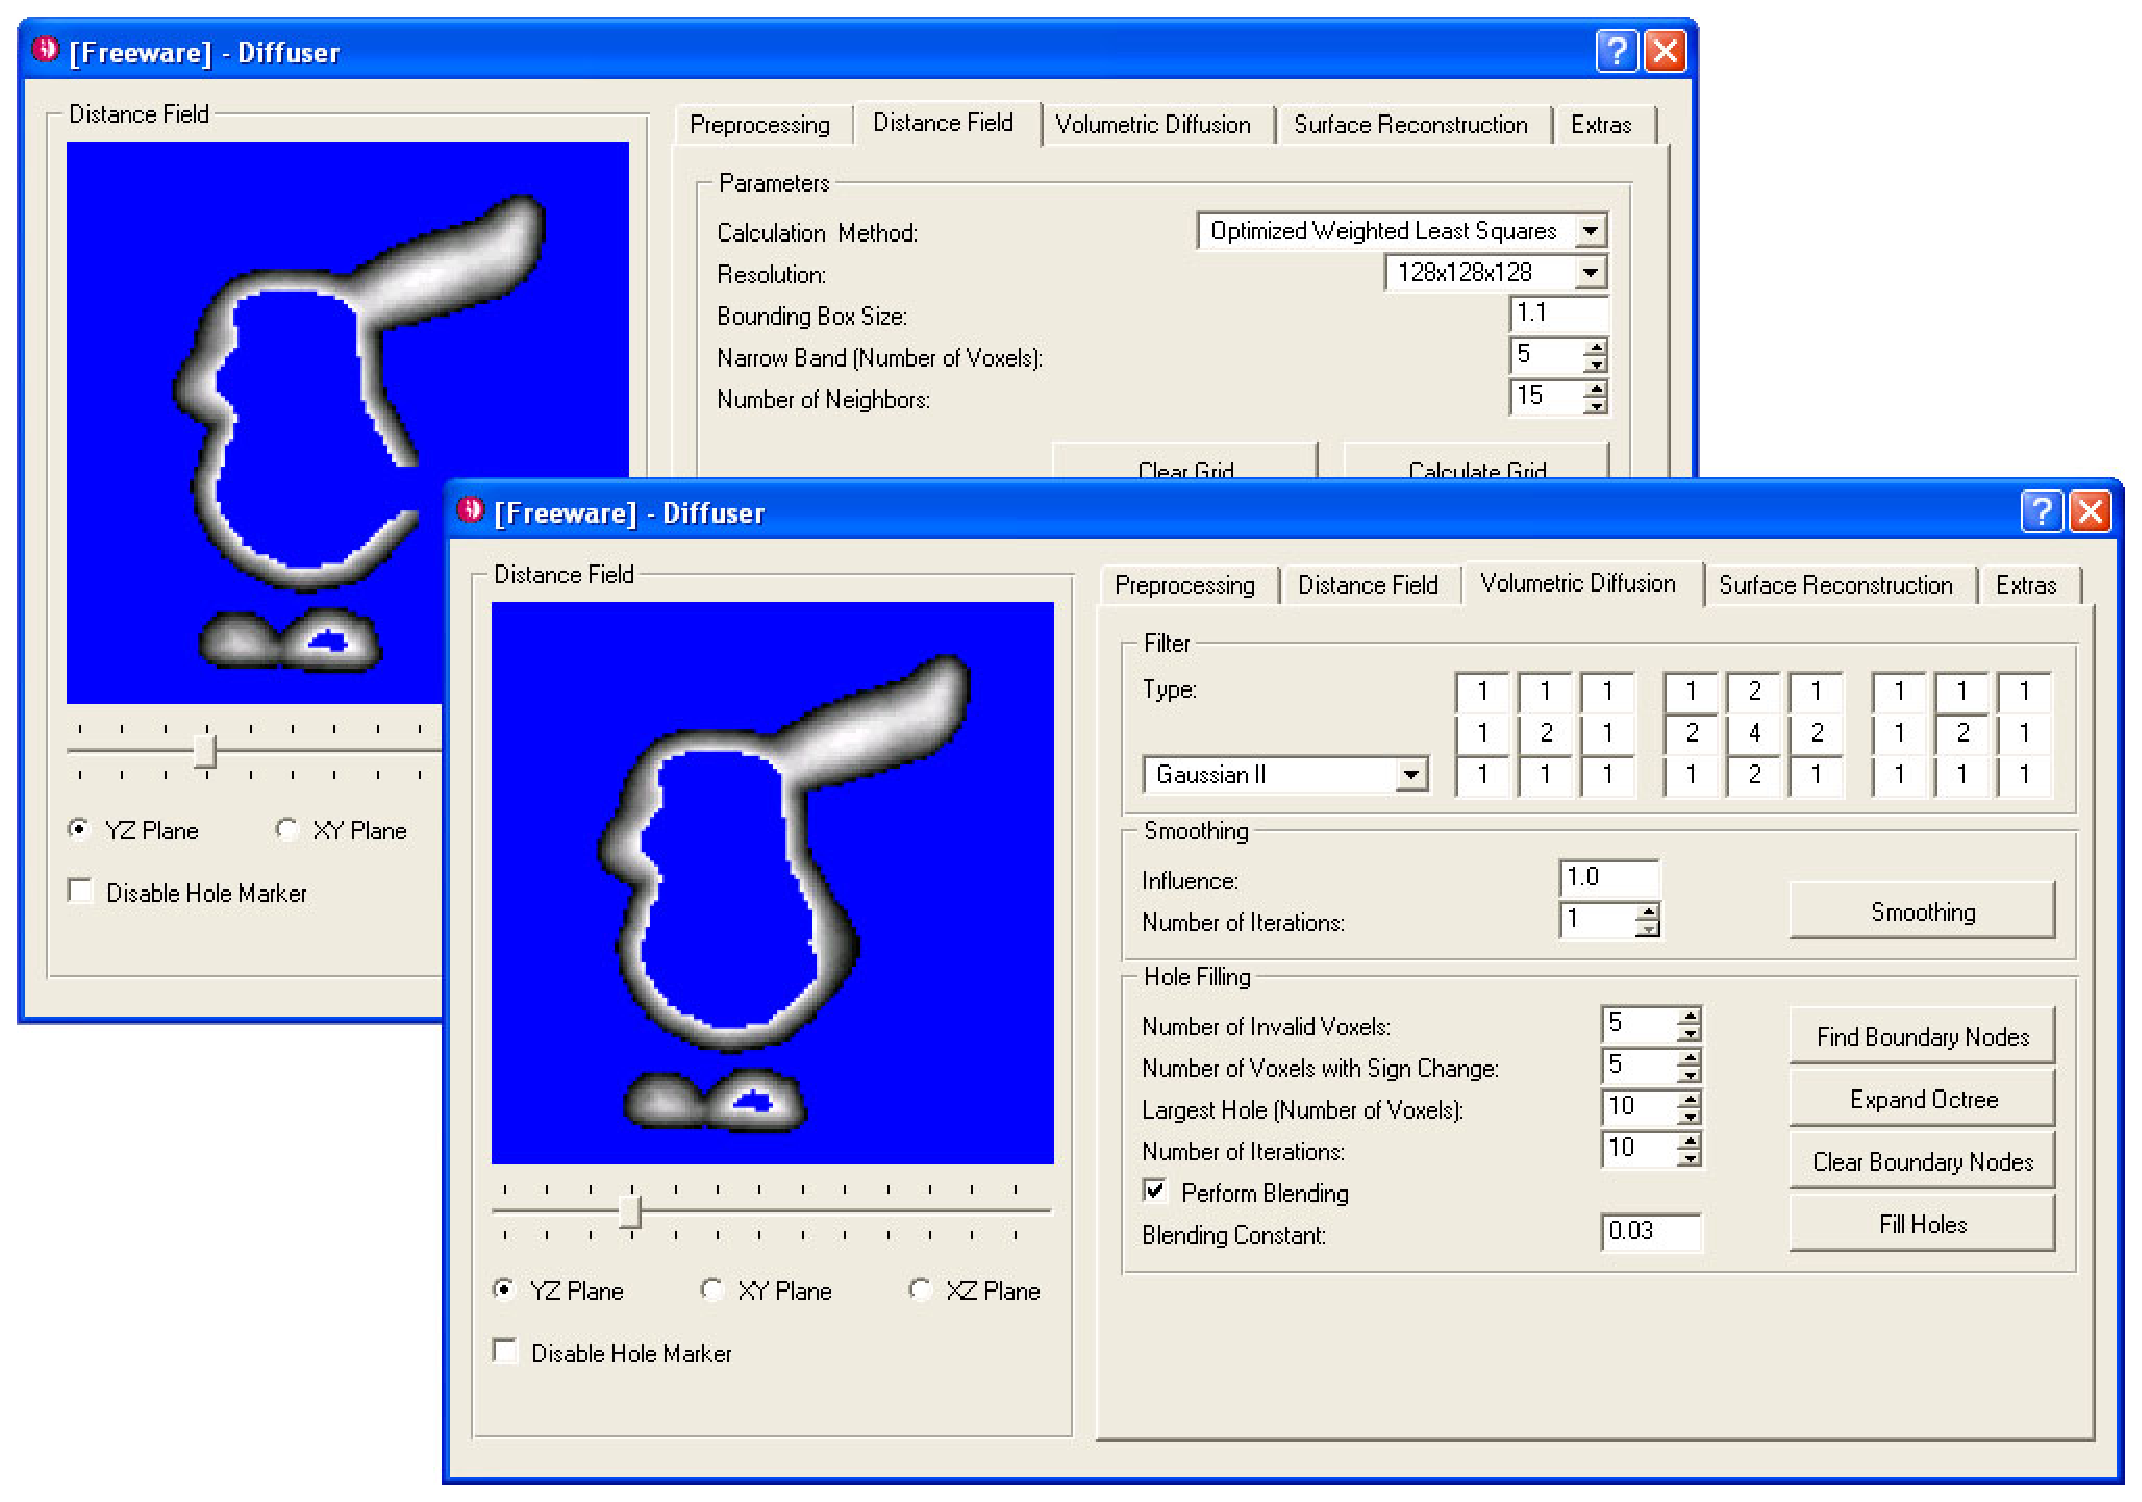
\includegraphics[width=0.45\textwidth]{figures/voldiff_ui}\label{fig:twofigures:voldiff_ui}}
     \caption{Comparison of steady state results. \protect\subref{fig:twofigures:IgeaNarrowBand} x method and \protect\subref{fig:twofigures:voldiff_ui} y method.}
     \label{fig:twofigures}
\end{figure}

